\documentclass{article}
% Change "article" to "report" to get rid of page number on title page
\usepackage{amsmath,amsfonts,amsthm,amssymb}
\usepackage{setspace}
\usepackage{Tabbing}
\usepackage{fancyhdr}
\usepackage{enumerate,lastpage}
\usepackage{extramarks}
\usepackage{chngpage}
\usepackage{soul,color,alltt}
\usepackage{graphicx,float,wrapfig}
\usepackage{multirow,comment}

% In case you need to adjust margins:
\topmargin=-0.45in      %
\evensidemargin=0in     %
\oddsidemargin=0in      %
\textwidth=6.5in        %
\textheight=9.0in       %
\headsep=0.25in         %

% Homework Specific Information
\newcommand{\hmwkTitle}{Curvature Prediction}
\newcommand{\hmwkClass}{}
\newcommand{\hmwkAuthorName}{Donglai\ Wei}


% Setup the header and footer
\pagestyle{fancy}                                                       %
\lhead{\hmwkAuthorName}                                                 %
\rhead{\firstxmark}                                                     %
\lfoot{\lastxmark}                                                      %
\cfoot{}                                                                %
\rfoot{Page\ \thepage\ of\ \pageref{LastPage}}                          %
\renewcommand\headrulewidth{0.4pt}                                      %
\renewcommand\footrulewidth{0.4pt}                                      %

% This is used to trace down (pin point) problems
% in latexing a document:
%\tracingall

%%%%%%%%%%%%%%%%%%%%%%%%%%%%%%%%%%%%%%%%%%%%%%%%%%%%%%%%\begin{enumerate}

% Some tools
\newcommand{\enterProblemHeader}[1]{\nobreak\extramarks{#1}{#1 continued on next page\ldots}\nobreak%
                                    \nobreak\extramarks{#1 (continued)}{#1 continued on next page\ldots}\nobreak}%
\newcommand{\exitProblemHeader}[1]{\nobreak\extramarks{#1 (continued)}{#1 continued on next page\ldots}\nobreak%
                                   \nobreak\extramarks{#1}{}\nobreak}%

\newlength{\labelLength}
\newcommand{\labelAnswer}[2]
  {\settowidth{\labelLength}{#1}%
   \addtolength{\labelLength}{0.25in}%
   \changetext{}{-\labelLength}{}{}{}%
   \noindent\fbox{\begin{minipage}[c]{\columnwidth}#2\end{minipage}}%
   \marginpar{\fbox{#1}}%

   % We put the blank space above in order to make sure this
   % \marginpar gets correctly placed.
   \changetext{}{+\labelLength}{}{}{}}%

\setcounter{secnumdepth}{0}
\newcommand{\homeworkProblemName}{}%
\newcounter{homeworkProblemCounter}%
\newenvironment{homeworkProblem}[1][Problem \arabic{homeworkProblemCounter}]%
  {\stepcounter{homeworkProblemCounter}%
   \renewcommand{\homeworkProblemName}{#1}%
   \section{\homeworkProblemName}%
   \enterProblemHeader{\homeworkProblemName}}%
  {\exitProblemHeader{\homeworkProblemName}}%

\newcommand{\problemAnswer}[1]
  {\noindent\fbox{\begin{minipage}[c]{\columnwidth}#1\end{minipage}}}%

\newcommand{\problemLAnswer}[1]
  {\labelAnswer{\homeworkProblemName}{#1}}

\newcommand{\homeworkSectionName}{}%
\newlength{\homeworkSectionLabelLength}{}%
\newenvironment{homeworkSection}[1]%
  {% We put this space here to make sure we're not connected to the above.
   % Otherwise the changetext can do funny things to the other margin

   \renewcommand{\homeworkSectionName}{#1}%
   \settowidth{\homeworkSectionLabelLength}{\homeworkSectionName}%
   \addtolength{\homeworkSectionLabelLength}{0.25in}%
   \changetext{}{-\homeworkSectionLabelLength}{}{}{}%
   \subsection{\homeworkSectionName}%
   \enterProblemHeader{\homeworkProblemName\ [\homeworkSectionName]}}%
  {\enterProblemHeader{\homeworkProblemName}%

   % We put the blank space above in order to make sure this margin
   % change doesn't happen too soon (otherwise \sectionAnswer's can
   % get ugly about their \marginpar placement.
   \changetext{}{+\homeworkSectionLabelLength}{}{}{}}%

\newcommand{\sectionAnswer}[1]
  {% We put this space here to make sure we're disconnected from the previous
   % passage

   \noindent\fbox{\begin{minipage}[c]{\columnwidth}#1\end{minipage}}%
   \enterProblemHeader{\homeworkProblemName}\exitProblemHeader{\homeworkProblemName}%
   \marginpar{\fbox{\homeworkSectionName}}%

   % We put the blank space above in order to make sure this
   % \marginpar gets correctly placed.
   }%

%%%%%%%%%%%%%%%%%%%%%%%%%%%%%%%%%%%%%%%%%%%%%%%%%%%%%%%%%%%%%



%%%%%%%%%%%%%%%%%%%%%%%%%%%%%%%%%%%%%%%%%%%%%%%%%%%%%%%%%%%%%
% Make title
\title{\vspace{0.3in}\textmd{\textbf{\hmwkTitle}}}
\date{2012.03.13}
%%%%%%%%%%%%%%%%%%%%%%%%%%%%%%%%%%%%%%%%%%%%%%%%%%%%%%%%%%%%%

\begin{document}
\begin{spacing}{1.1}
\maketitle

\section{0. Visualize FCW signal on Google Map}
Some are fired on straight roads where there may be cars closed by.
But some are triggered at the turning point of the road with big curvature, which may well be false positive.\\\\
http://projects.csail.mit.edu/drivehistory/index.php?id=99
\begin{figure}
  \centering
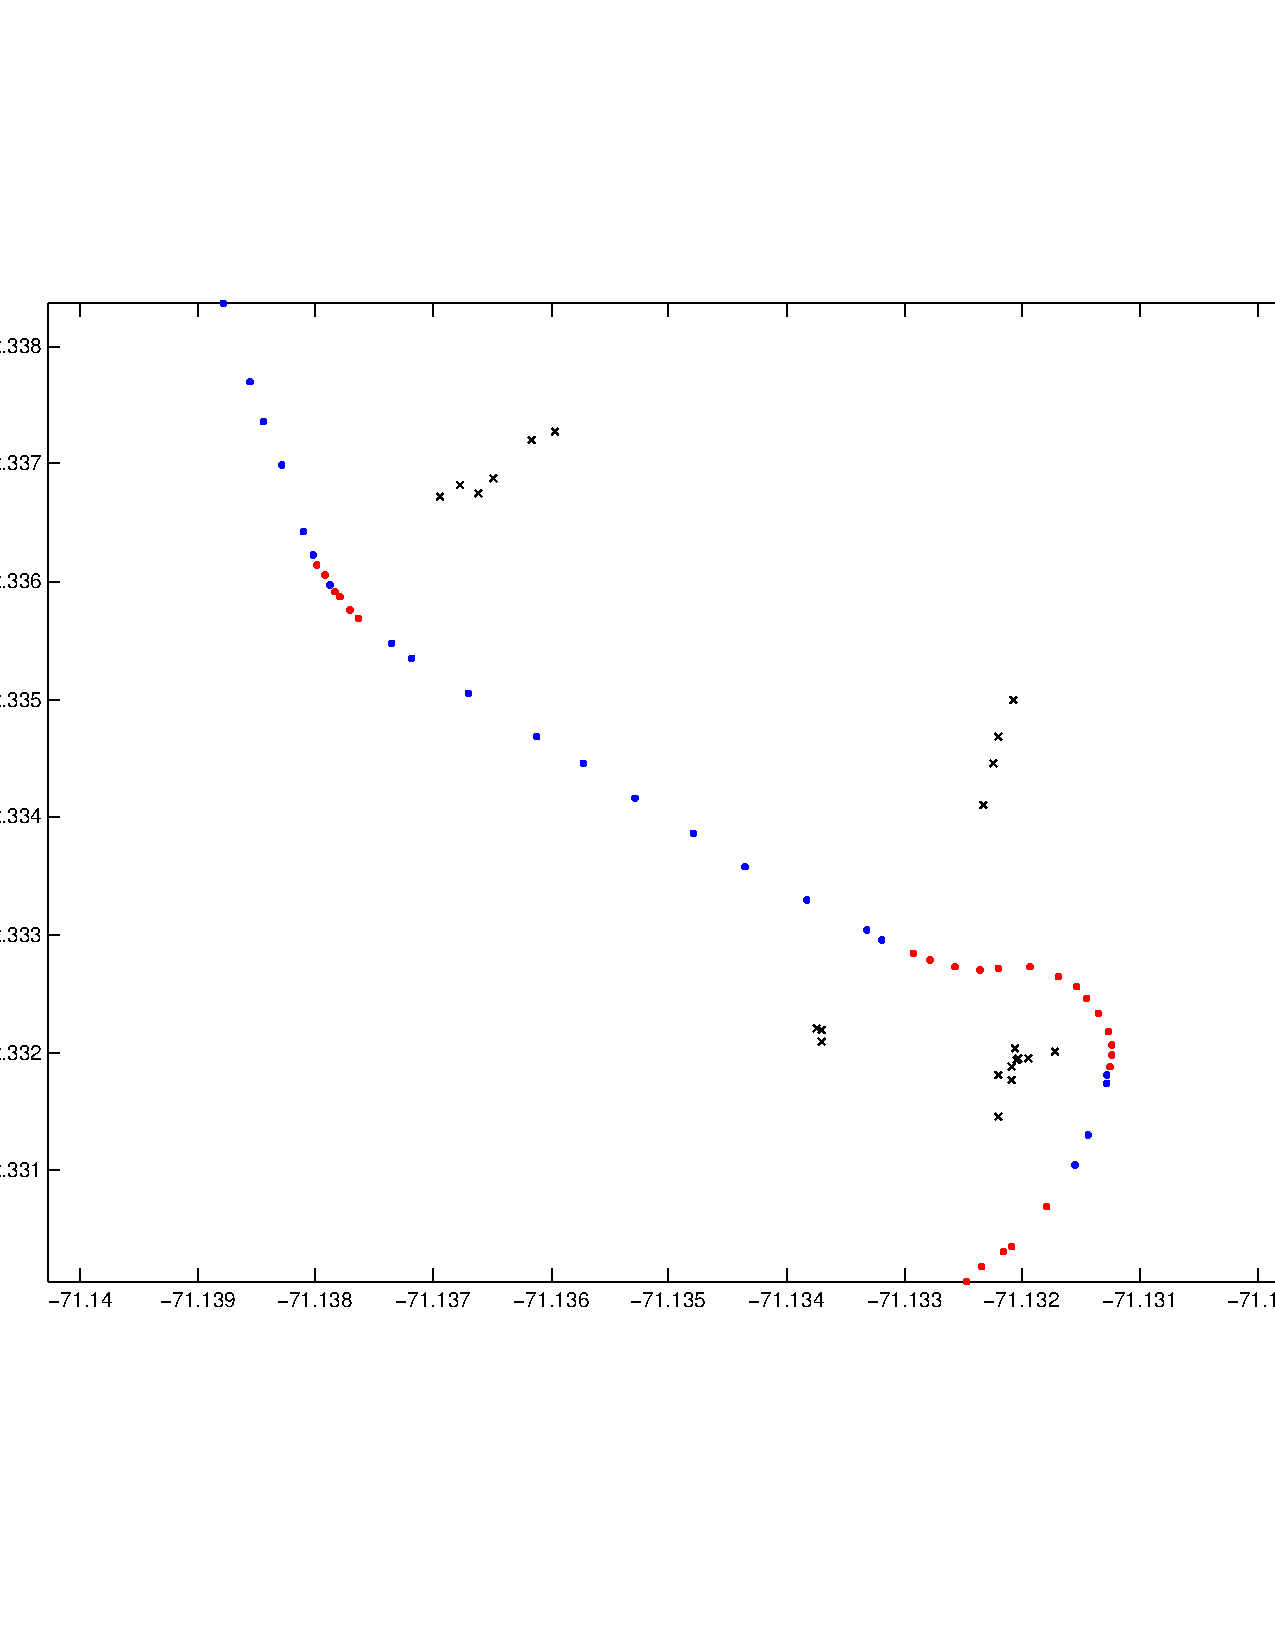
\includegraphics[width=3in,height=3in]{rd.pdf}
\caption{Interesting Points clustered}
\end{figure}
\begin{figure}
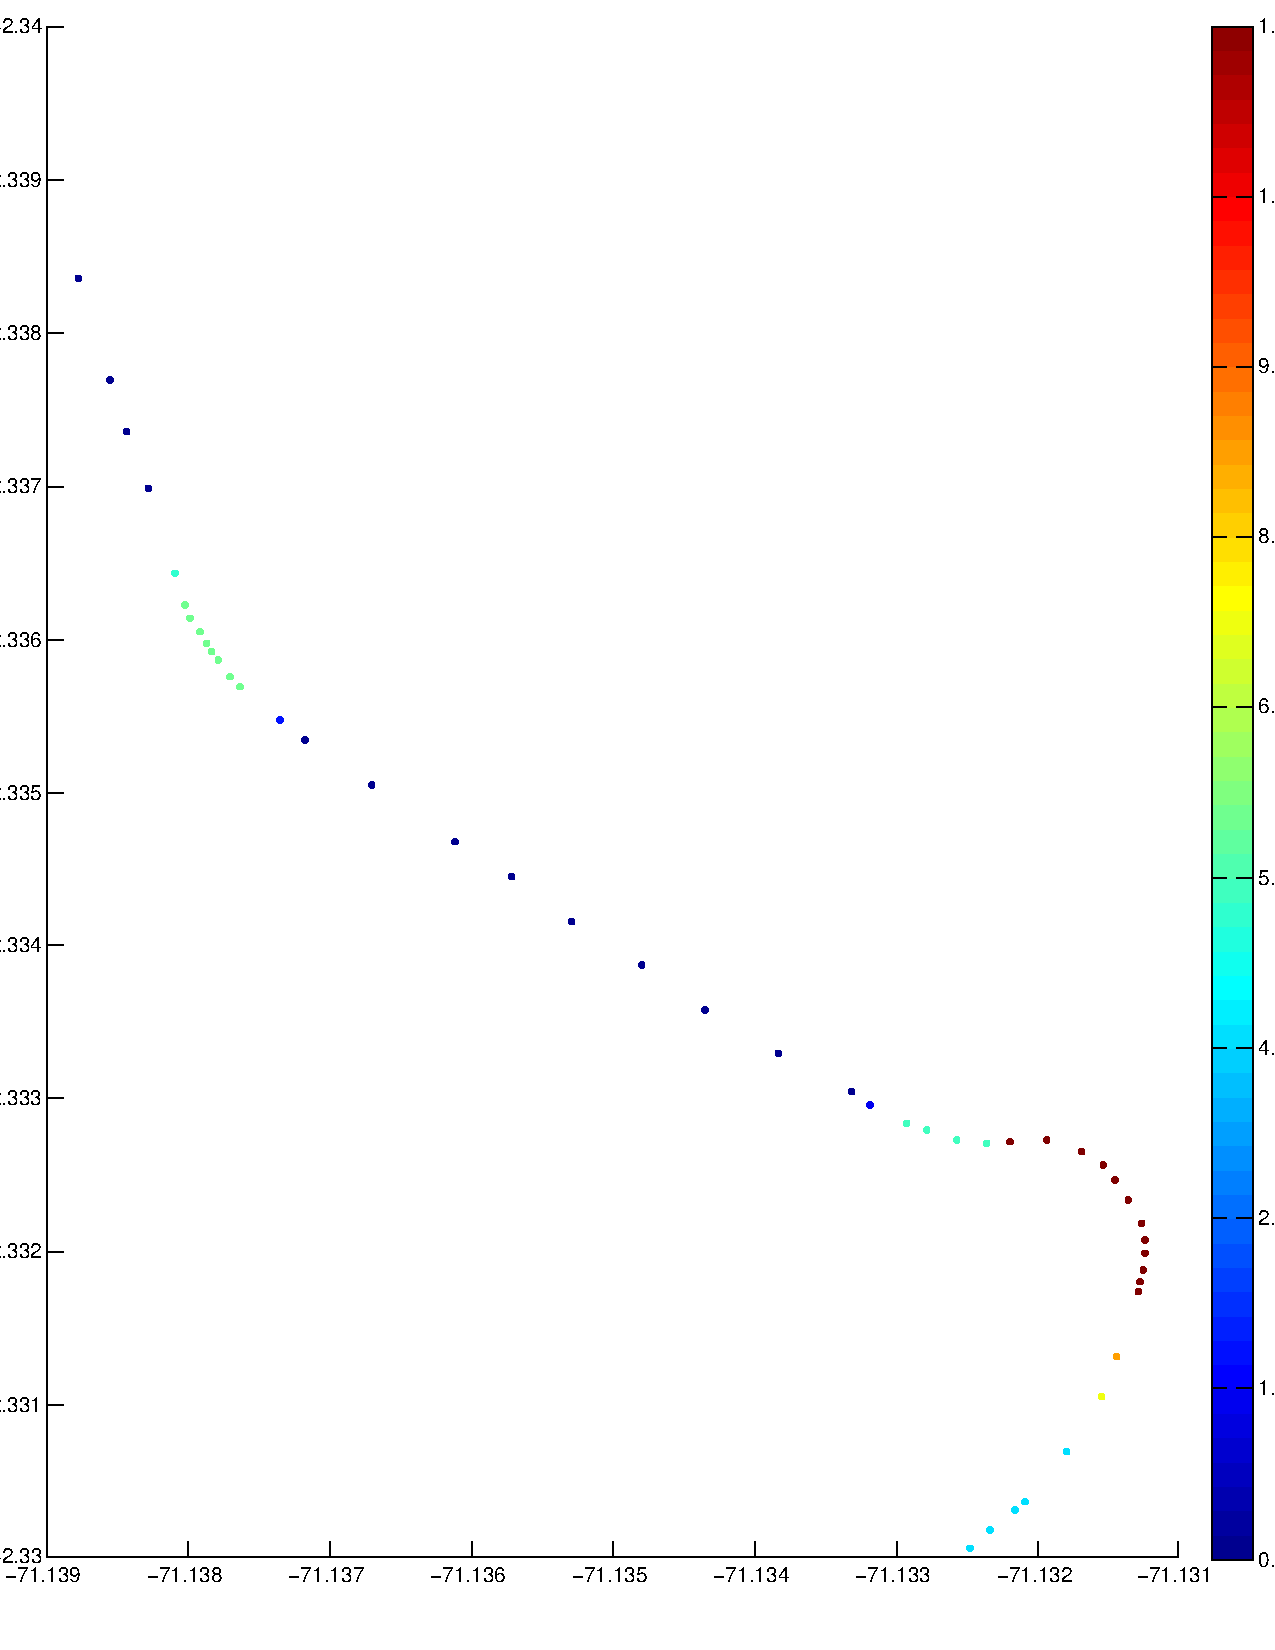
\includegraphics[width=3in,height=3in]{rd2.pdf}
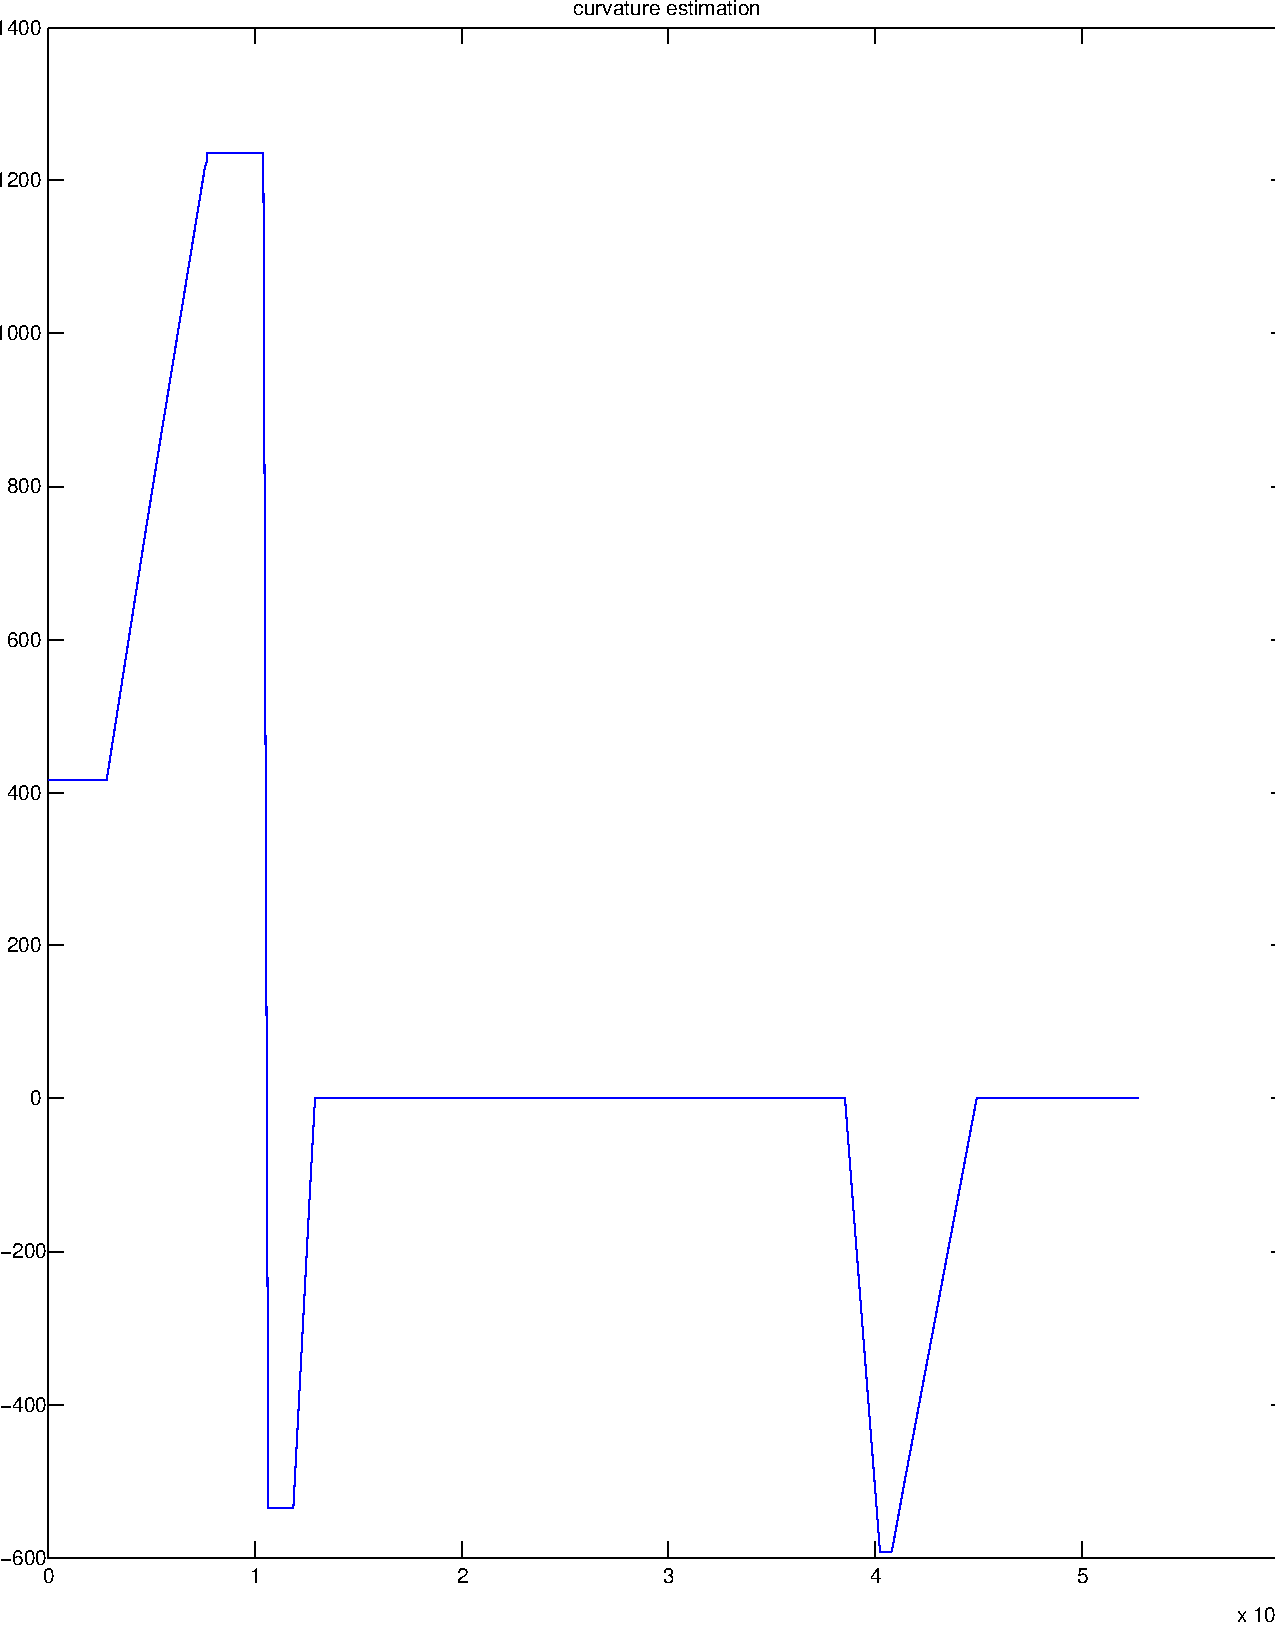
\includegraphics[width=3in,height=3in]{curvature.pdf}
\caption{color-coded curvature map(left) and piecewise curvature plot(right)}
\end{figure}
\begin{figure}
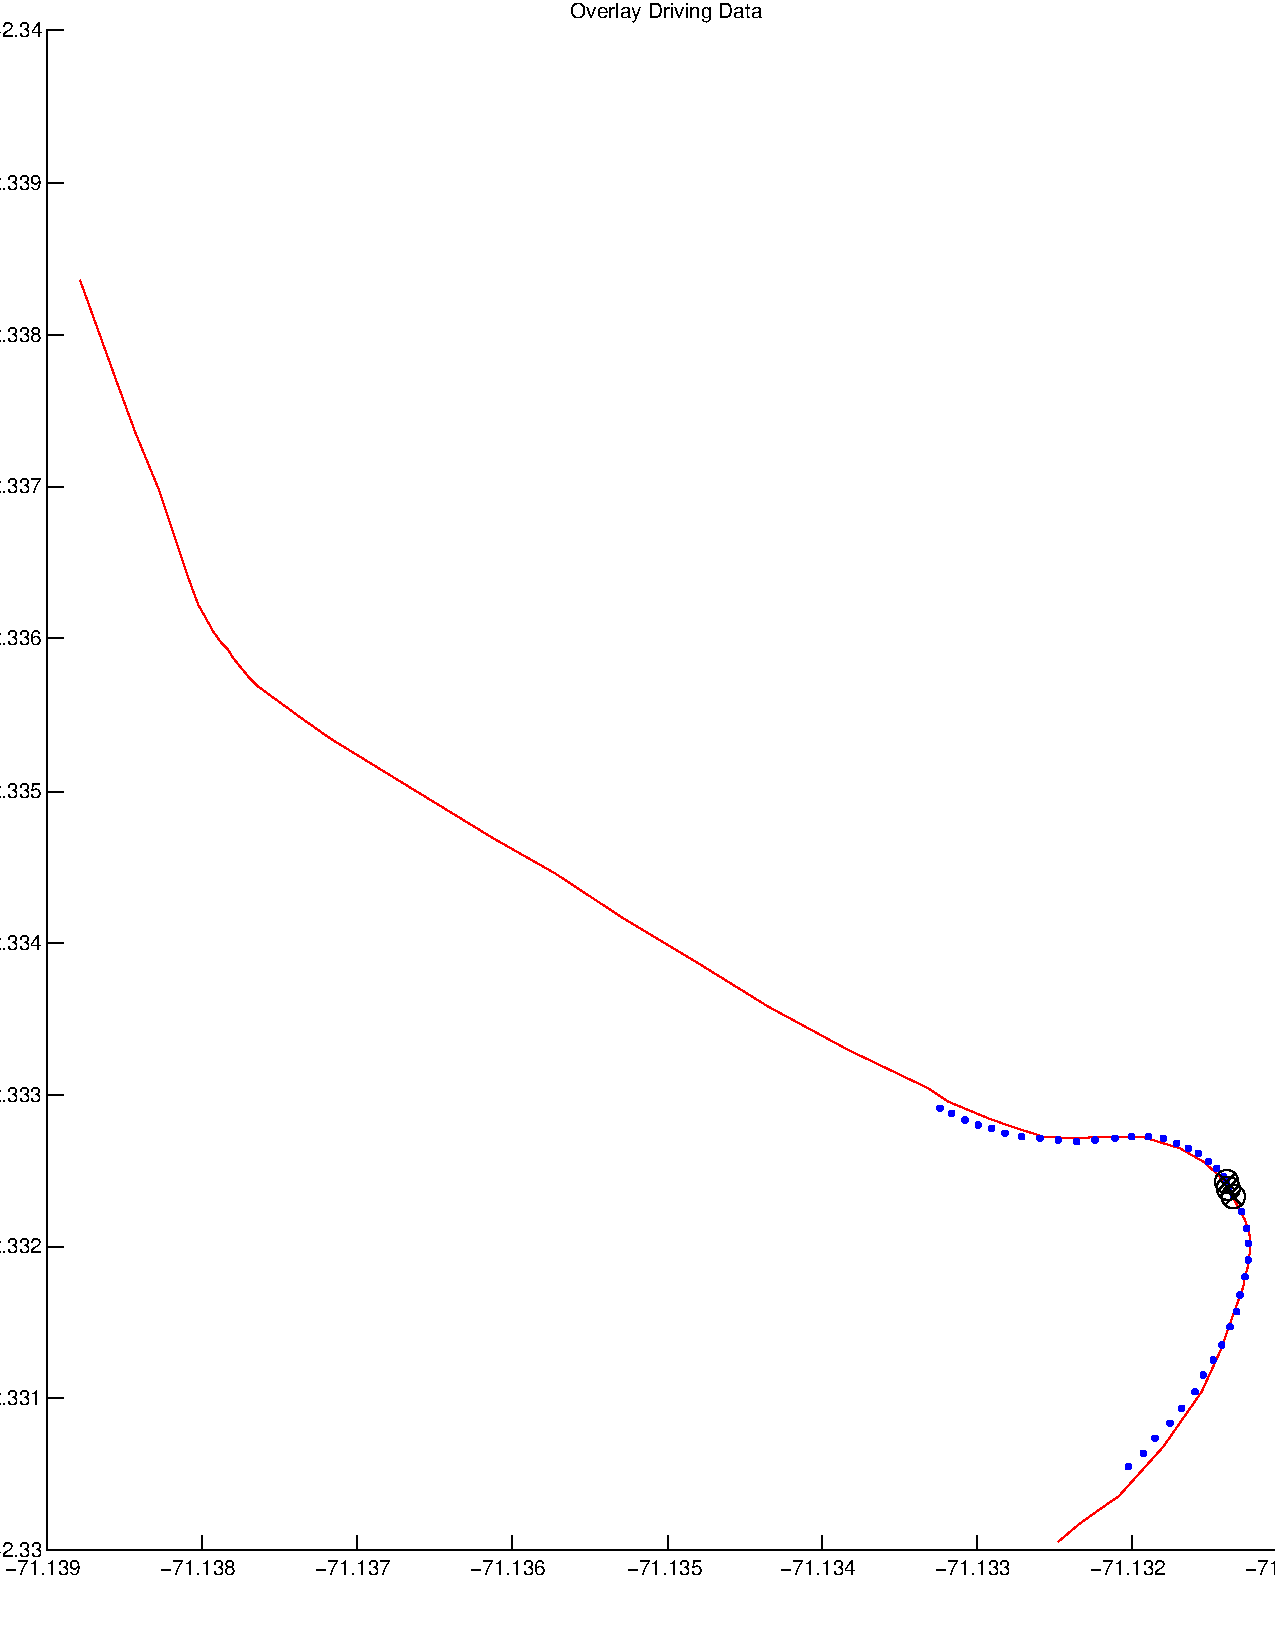
\includegraphics[width=3in,height=3in]{data.pdf}
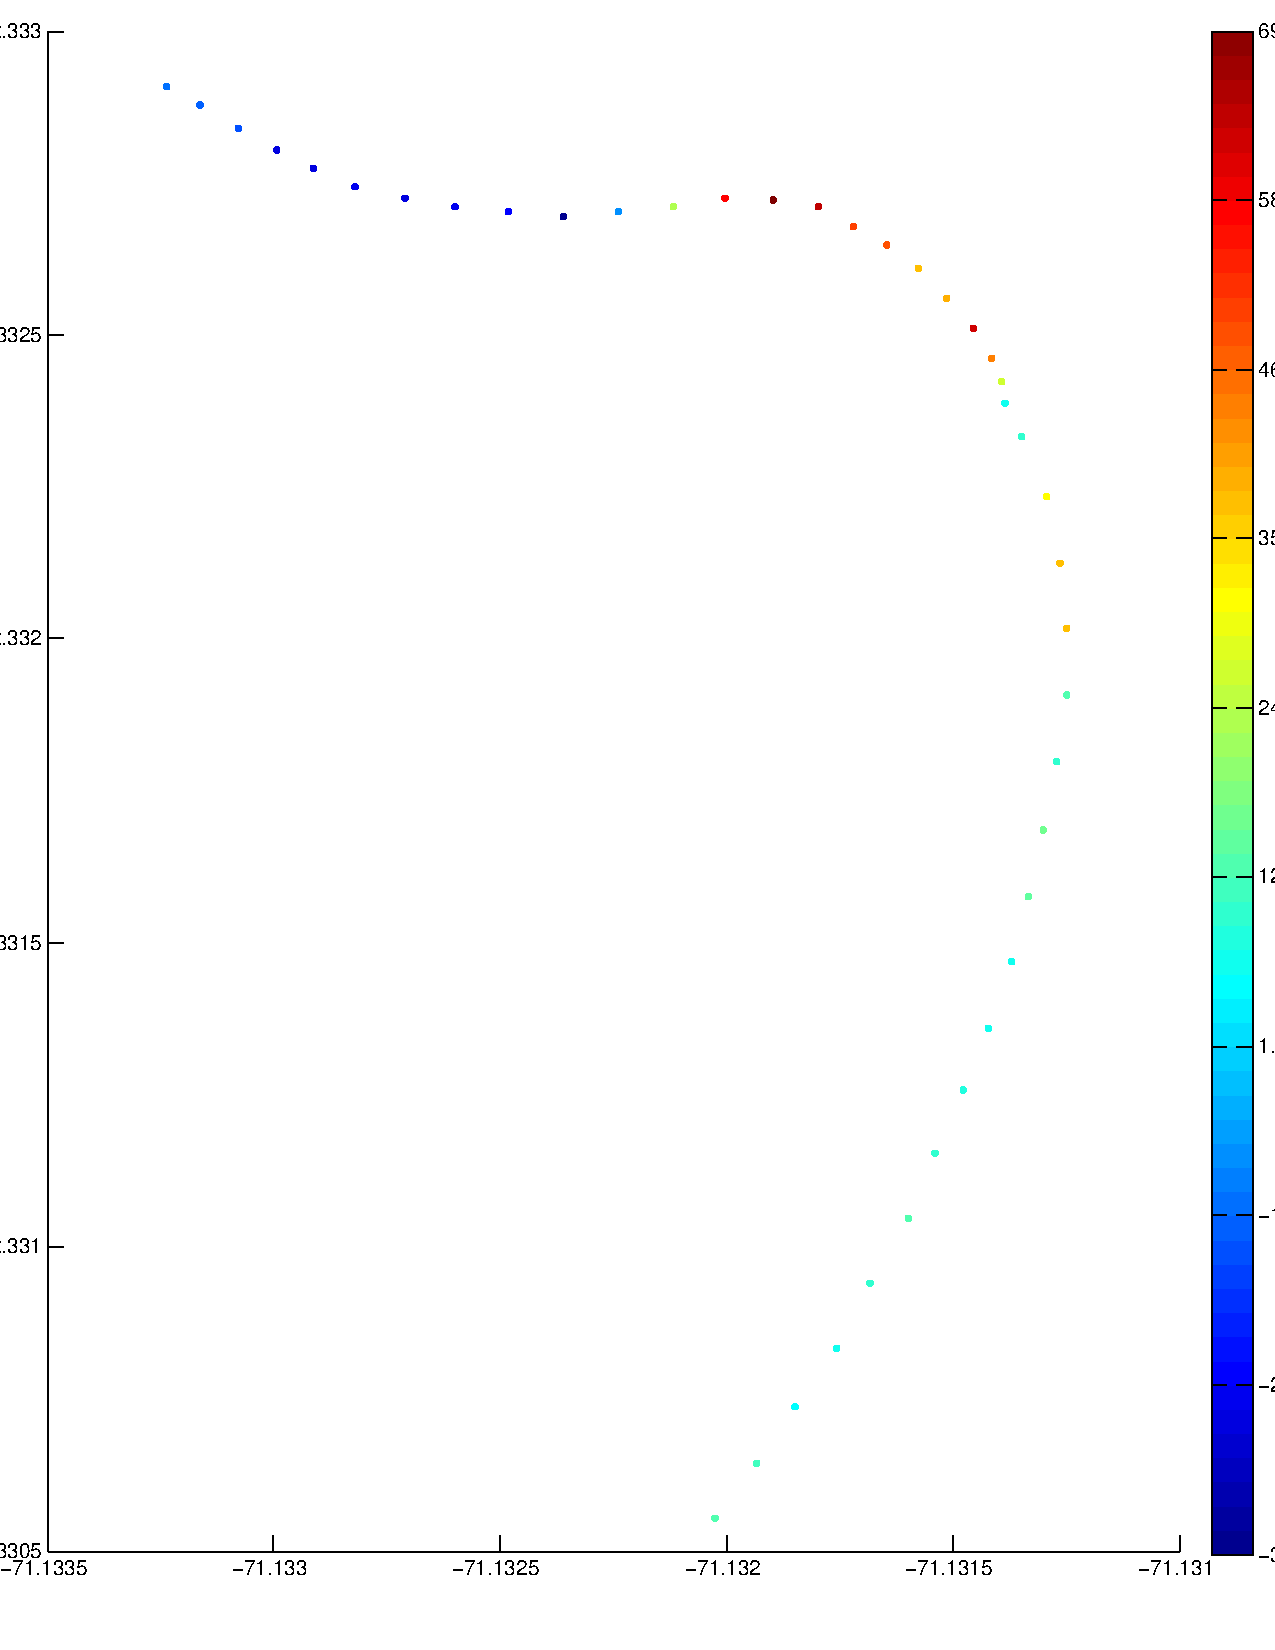
\includegraphics[width=3in,height=3in]{steer.pdf}
\caption{Overlayed gps data (left) and color-coded steering wheel angle(right)}

\end{figure}

\begin{comment}
\end{comment}
\section{1. Curvature Prediction}
\subsection{1.0 Database}
Suppose at the current moment, we know exactly positions of the car within the next one minute, then curvature prediction can be done by looking up the precomputed and saved curvature of these positions on the map. Here, we engineer a robust procedure to estimate curvature for each position on the map (OpenStreetMap, OSM).\\\\
Below, we demonstrate our method on a road segment where the FCW signal triggers.
\begin{enumerate}[(a)]
\item Local Model:\\
There are two ways to estimate the curvature of a point on the curve: one deals with the change of the gradient of the curve and the other fits an oscillating circle tangent to the gradient at the point. Since the map data itself are noisy, the second order estimation is not robust in the first approach, causing significant discontinuity of the estimation. Thus, we take the second approach where each oscillating circle is estimated from the neighborhood of the point.
\item Cluster Interesting Points: \\
We first filter out points with small curvatures where the curve is close to a line. Then we try to cluster the center of the oscillating circles of the rest points which contribute to significant bended curves.

\item Global Model:\\
According to ~\cite{}, we can assume a Piecewise Linear Curvature Model for our road segment due to the principles of road construction. Above, we've segmented out bended part of the curve and we just need to  
\end{enumerate}

\subsection{1.1) Time Independent Model}
\subsection{1.2) Time Dependent Model: HMM/KF}
\subsection{1.3) Incorporating Road Network}
\begin{comment}
\begin{figure}[h]
\caption{independent MoG model}
  \centering
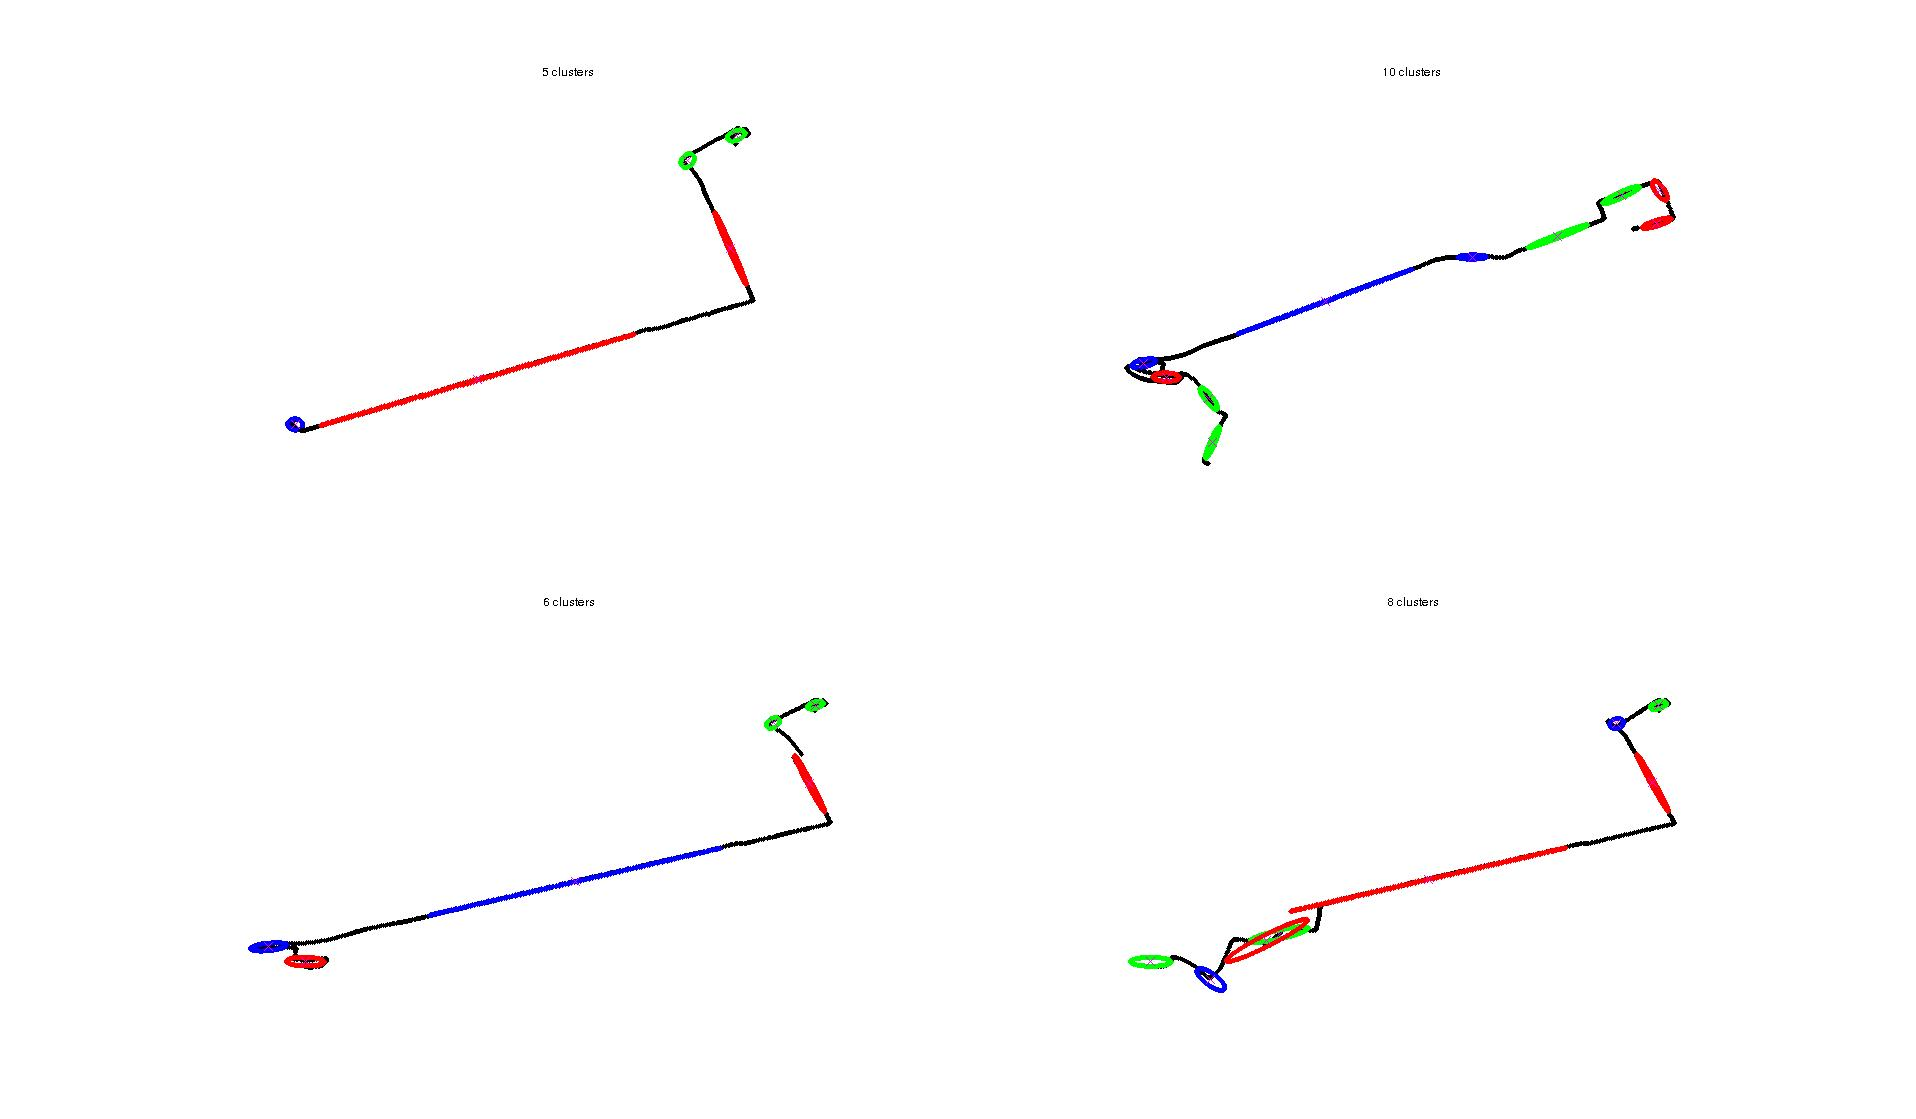
\includegraphics[width=3in,height=4in]{ind_cluster.jpg}
\end{figure}
\end{comment}



\end{spacing}
\end{document}

%%%%%%%%%%%%%%%%%%%%%%%%%%%%%%%%%%%%%%%%%%%%%%%%%%%%%%%%%%%%%
